\section{Definisi HTTP Post Method}
POST merupakan metode permintaan dari HTTP yang digunakan untuk mengirim data ke server untuk membuat / memperbarui sumber daya. Biasanya metode POST digunakan untuk menggugah file atau mengirimkan  formulir web yang sudah diisi. 

Metode POST digunakan untuk mengirimkan entitas ke sumber daya yang ditentukan, sering menyebabkan perubahan status atau efek samping pada server. Data akan dikirim ulang (browser harus memberi tahu pengguna bahwa data akan dikirim ulang). Metode POST tidak dapat di bookmark juga tidak terdapat  cache. Jika menggunakan metode POST parameternya tidak akan tersimpan di browser history, ini membuat metode POST lebih aman untuk digunakan karena, informasi penting..rahasia tidak dapat diakses secara ilegal.

\section{Mekanisme HTTP Post Method}
Metode POST mentransfer informasi melalui HTTP. Informasi dikodekan dan dimasukkan ke dalam header yang disebut QUERY\_STRING. Data untuk metode POST sama seperti yang dikirimkan melalui formulir HTTP. Kemudian Agen internal mengekstrak bidang dari setiap formulir dan setiap aliran Post ke tabel aliran data. Namun data tidak akan ditampilakn pada header.

HTTP POST dapat terjadi sebagai hasil dari pengguna yang mengirimkan formulir HTML yang berisi bidang <INPUT>, atau POST dapat dibuat dengan menggunakan HTTP sebagai protokol komunikasinya.

\section{Contoh  URL HTTP Post Method}
\lstinputlisting[caption=Skrip Fungsi Contoh HTTP POST,label={lst:fhp}]{src/11/fhp.py}

Listing \ref{lst:fhp} merupakan contoh dari HTTP POST pada flask. Route disini berfungsi untuk menautkan URL ke suatu fungsi yang telah didefinisikan. Show\_index() merupakan fungsi yang digunakan untuk menampilkan gambar kedalam template HTML yang dapat diakses lewat browser. Cara menjalankannya seperti berikut : 
\begin{enumerate}
\item Buka terminal pada text editor yang dimiliki pada PC ataupun menggunakan CMD. Pada tutorial ini menggunakan terminal pada text editor Visual Code seperti pada gambar \ref{fig:tvc}.
\begin{figure}[!htbp]
	\centerline{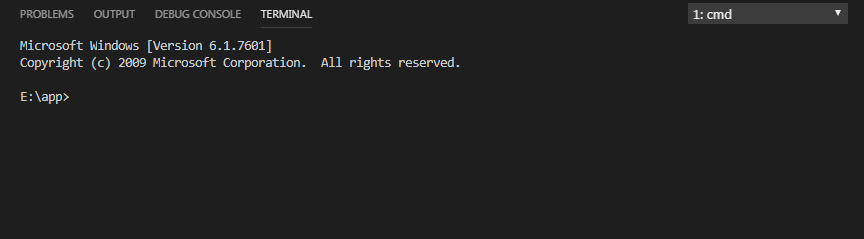
\includegraphics[width=0.85\textwidth]{figures/11/tvc.PNG}}
	\caption{Terminal Pada Visual Code}
	\label{fig:tvc}
\end{figure}

\item Buka Folder dimana file codingan tadi tersimpan seperti pada gambar \ref{fig:flc}.
\begin{figure}[!htbp]
	\centerline{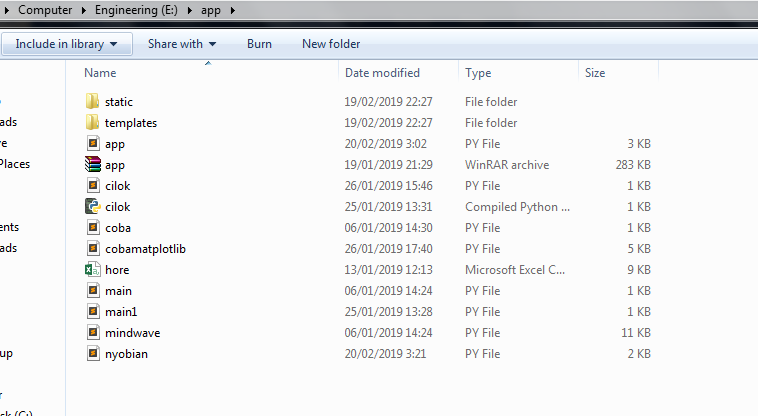
\includegraphics[width=0.85\textwidth]{figures/11/flc.PNG}}
	\caption{Folder Lokasi Codingan}
	\label{fig:flc}
\end{figure}

\item Buka Folder tadi Di Terminal dengan mengetikan “cd E:/app maka akan masuk ke folder tersebut.
\item Kemudian untuk menjalankan aplikasinya ketikan “python app.py” app.py merupakan file codingan python yang berisikan Skrip Fungsi diatas. Maka ketika dijalankan akan muncul hasil seperti pada gambar \ref{fig:ja}.
\begin{figure}[!htbp]
	\centerline{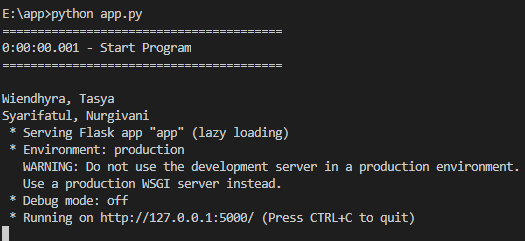
\includegraphics[width=0.85\textwidth]{figures/11/ja.PNG}}
	\caption{Menjalankan Aplikasi}
	\label{fig:ja}
\end{figure}

\item Terdapat link dari hasil menjalankan tadi, kemudian salin link tersebut ke web browser anda. Maka hasilnya akan seperti pada gambar \ref{fig:chp}.
\begin{figure}[!htbp]
	\centerline{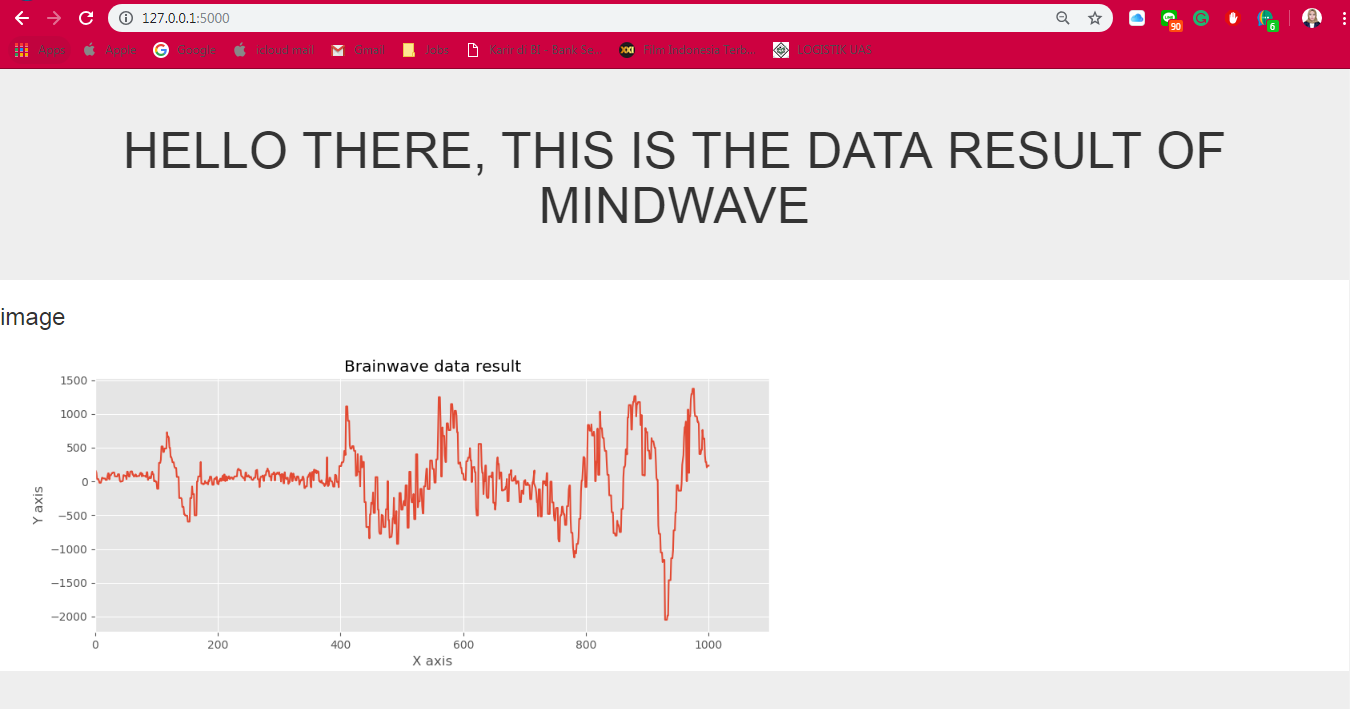
\includegraphics[width=0.85\textwidth]{figures/11/chp.PNG}}
	\caption{Contoh HTTP POST}
	\label{fig:chp}
\end{figure}
\end{enumerate}

\section{Definisi HTTP Put}
Metode permintaan HTTP PUT membuat resource baru atau menggantikan representasi resource target dengan muatan permintaan. Perbedaan antara PUT dan POST adalah bahwa PUT idempoten: menyebutnya sekali atau beberapa kali berturut-turut memiliki efek yang sama (yaitu tidak berpengaruh), di mana POST identik yang berurutan dapat memiliki efek tambahan, seperti mengirimkan pesan beberapa kali.

\section{Mekanisme HTTP Put Method}
Cara kerja dari PUT ini hampir sama dengan POST. Namun ketika pada saat mengirimkan request dan jika resource target tidak memiliki representasi saat ini dan permintaan PUT berhasil membuatnya, maka server asal harus memberi tahu agen pengguna dengan mengirimkan respons 201 (Created). Dan apabila request yang dikirimkan sudah ada maka akan dilakukan update data.

\section{Contoh URL HTTP Put Method}
\lstinputlisting[caption=Skrip Fungsi Contoh HTTP PUT,label={lst:chp}]{src/11/chp.py}

Listing \ref{lst:chp} merupakan contoh dari HTTP PUT yang digunakan untuk mengupdate hasil dari fungsi yang telah didefinisikan menggunakan metode GET sebelumnya. Fungsinya seperti pada listing \ref{lst:fhg}:
\lstinputlisting[caption=Skrip Fungsi Pada HTTP GET,label={lst:fhg}]{src/11/fhg.py}

\section{Definisi HTTP Delete}
Sesuai dengan namanya yaitu delete yang berarti menghapus resource yang dituju. Metode DELETE meminta server asal menghapus sumber yang diidentifikasi oleh Request-URI. Metode ini dapat ditimpa oleh intervensi manusia (atau cara lain) pada server asal. Klien tidak dapat menjamin bahwa operasi telah dilakukan, bahkan jika kode status dikembalikan dari server asal menunjukkan bahwa tindakan telah berhasil diselesaikan.

\section{Mekanisme HTTP Delete Method}
Ketika dilakukan request dengan menggunakan metode DELETE, maka Request-URI akan melakukan identifikasi dan meminta untuk menghapus sumber yang dituju. DELETE. Bisa saja terdapat respon pada saat penghapusan sumber/data dan bisa juga tidak ada respon namun data/sumber berhasil dihapus ketika dilakukan pengecekan.

\section{Contoh URL HTTP Delete Method}
\lstinputlisting[caption=Skrip Fungsi Pada HTTP DELETE,label={lst:fhd}]{src/11/fhd.py}

Listing \ref{lst:fhd} akan menghapus data yang terdapat pada fungsi yang sebelumnya.

\section{Instalasi Dan Tata Cara Penggunaan Postman Untuk HTTP Post, Put Dan Delete} 
Postman merupakan klien HTTP yang digunakan untuk melakukan tes terhadap web service. Postman sendiri dapat diinstal langsung pada PC ataupun diinstal pada web browser yang mendukung. Kali ini akan dibuat sebuah tutorial cara menginstal Postman di PC serta pada web browser.
\subsection{Instalasi Postman Di PC}
\begin{enumerate}
\item Untuk menginstal Postman, berkasnya dapat diunduh di https://www.getPostman.com/downloads/ . unduh sesuai dengan Sistem Operasi yang anda gunakan, untuk tutorial ini menggunakan Windows seperti pada gambar \ref{fig:wp}.
\begin{figure}[!htbp]
	\centerline{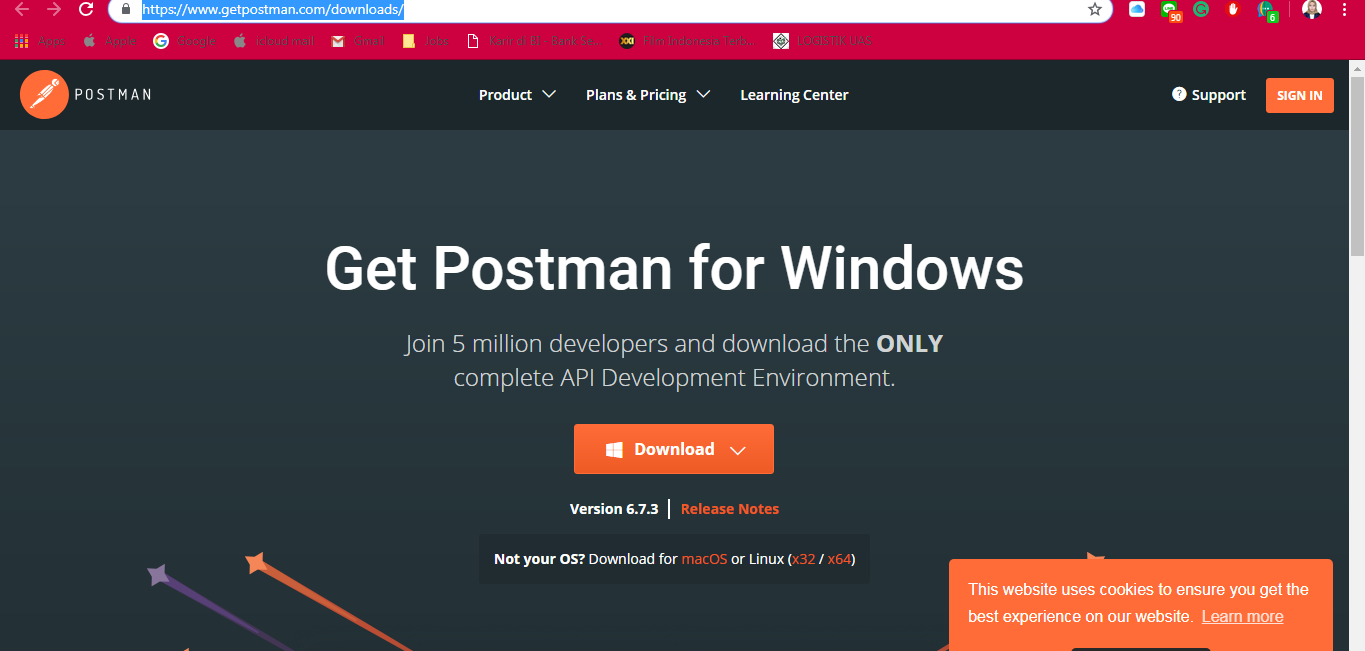
\includegraphics[width=0.85\textwidth]{figures/11/wp.PNG}}
	\caption{Website Postman}
	\label{fig:wp}
\end{figure}

\item Unduh versi Windows 64 bit, karena pada tutorial ini menggunakan Windows 64 bit. Jika Anda memiliki Windows 32 bit, Anda dapat mengunduh Postman untuk Windows 64 bit seperti yang ditunjukkan seperti pada gambar \ref{fig:pvw}.
\begin{figure}[!htbp]
	\centerline{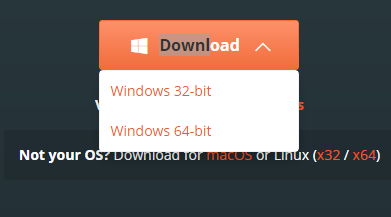
\includegraphics[width=0.85\textwidth]{figures/11/pvw.PNG}}
	\caption{Postman Versi Windows 64-bit}
	\label{fig:pvw}
\end{figure}

\item Setelah diunduh, Anda dapat menemukan file yang diunduh di lokasi unduhan default sistem Anda. Jika Anda menggunakan browser Chrome, file yang diunduh akan muncul di bagian bawah browser seperti yang ditunjukkan seperti pada gambar \ref{fig:bfi}.
\begin{figure}[!htbp]
	\centerline{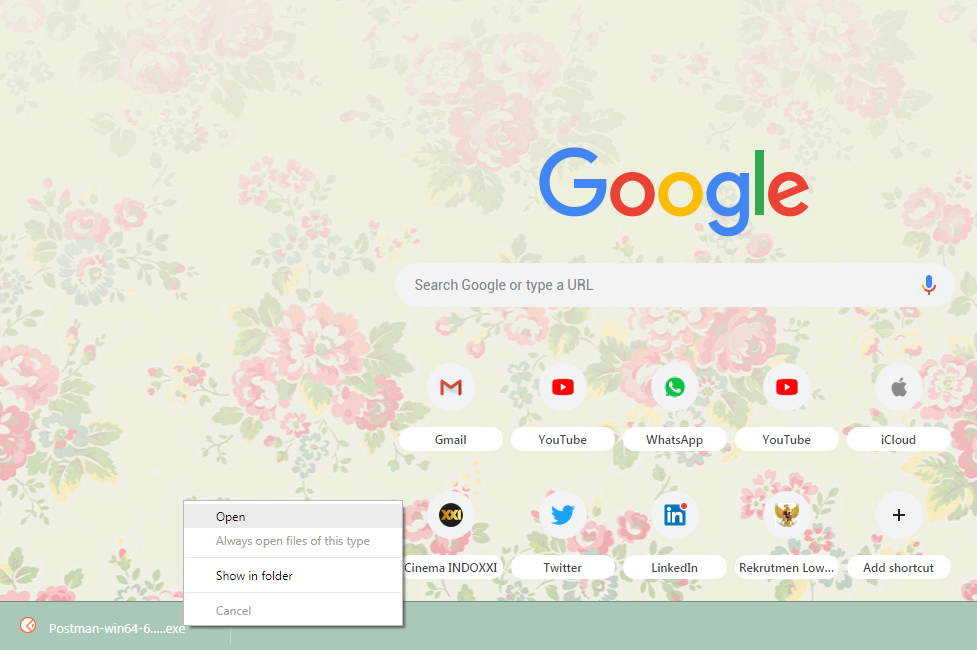
\includegraphics[width=0.85\textwidth]{figures/11/bfi.PNG}}
	\caption{Buka File Instalasi}
	\label{fig:bfi}
\end{figure}

\item Buka file exe Postman Windows 64 bit untuk instalasi pada sistem anda. Dan lakukan instalasi seperti pada gambar \ref{fig:ip}.
\begin{figure}[!htbp]
	\centerline{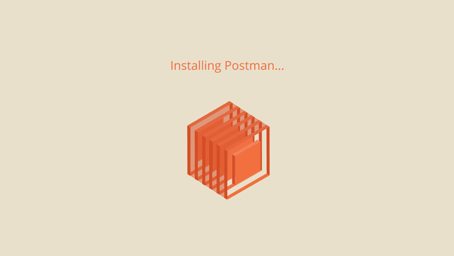
\includegraphics[width=0.85\textwidth]{figures/11/ip.PNG}}
	\caption{Instalasi Postman}
	\label{fig:ip}
\end{figure}

\item Tunggu sampai proses instalasi selesai.
\item Setelah proses instalasi selesai, akan diminta untuk membuat akun seperti pada gambar \ref{fig:hap}.
\begin{figure}[!htbp]
	\centerline{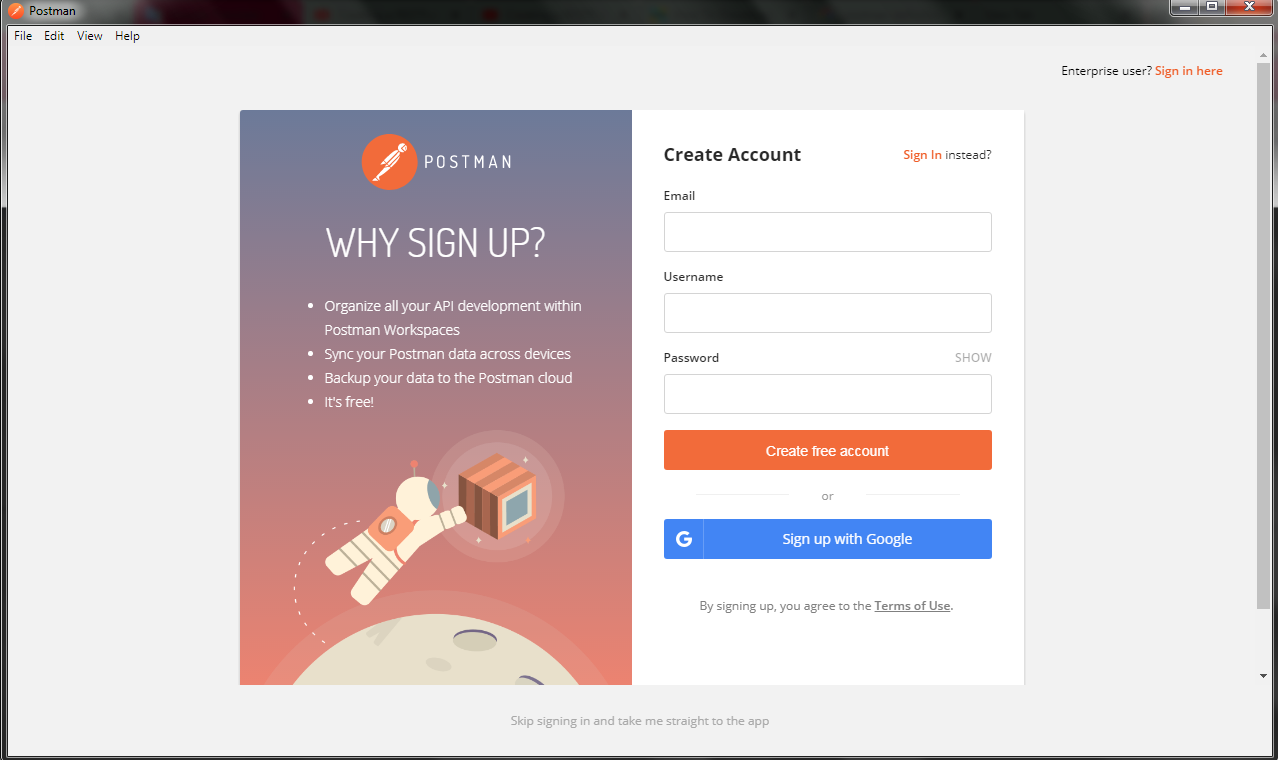
\includegraphics[width=0.85\textwidth]{figures/11/hap.PNG}}
	\caption{Halaman Membuat Akun Postman}
	\label{fig:hap}
\end{figure} 

\item Pilih lah membuat akun dengan akun Google anda yaitu dengan klik tombol “ Sign Up With Google”. Anda akan diminta untuk login ke akun google anda. Silahkan isi klom email dan password sesuai dengan akun google yang anda miliki seperti pada gambar \ref{fig:lpg}.
\begin{figure}[!htbp]
	\centerline{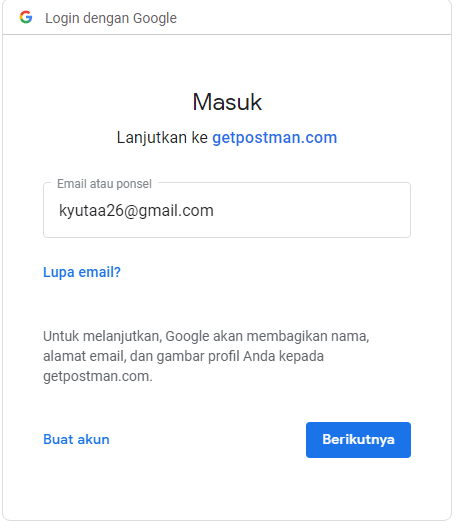
\includegraphics[width=0.85\textwidth]{figures/11/lpg.PNG}}
	\caption{Login Postman Dengan Akun Google}
	\label{fig:lpg}
\end{figure}

Password seperti pada gambar \ref{fig:plg}.
\begin{figure}[!htbp]
	\centerline{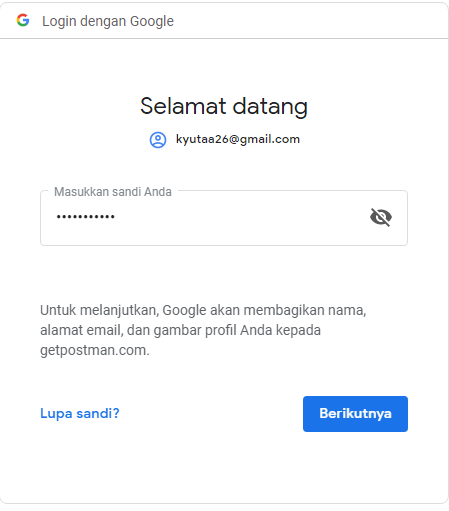
\includegraphics[width=0.85\textwidth]{figures/11/plg.PNG}}
	\caption{Password Untuk Login Postman Dengan Akun Google}
	\label{fig:plg}
\end{figure}
 
\item Klik berikutnya untuk menyelesaikan proses login. Ini akan secara otomatis membuka Alat Postman. Setelah instalasi dan pendaftaran berhasil (daftar dengan Gmail Anda), Anda bisa melihat toolkit Postman seperti pada gambar \ref{fig:tp}.
\begin{figure}[!htbp]
	\centerline{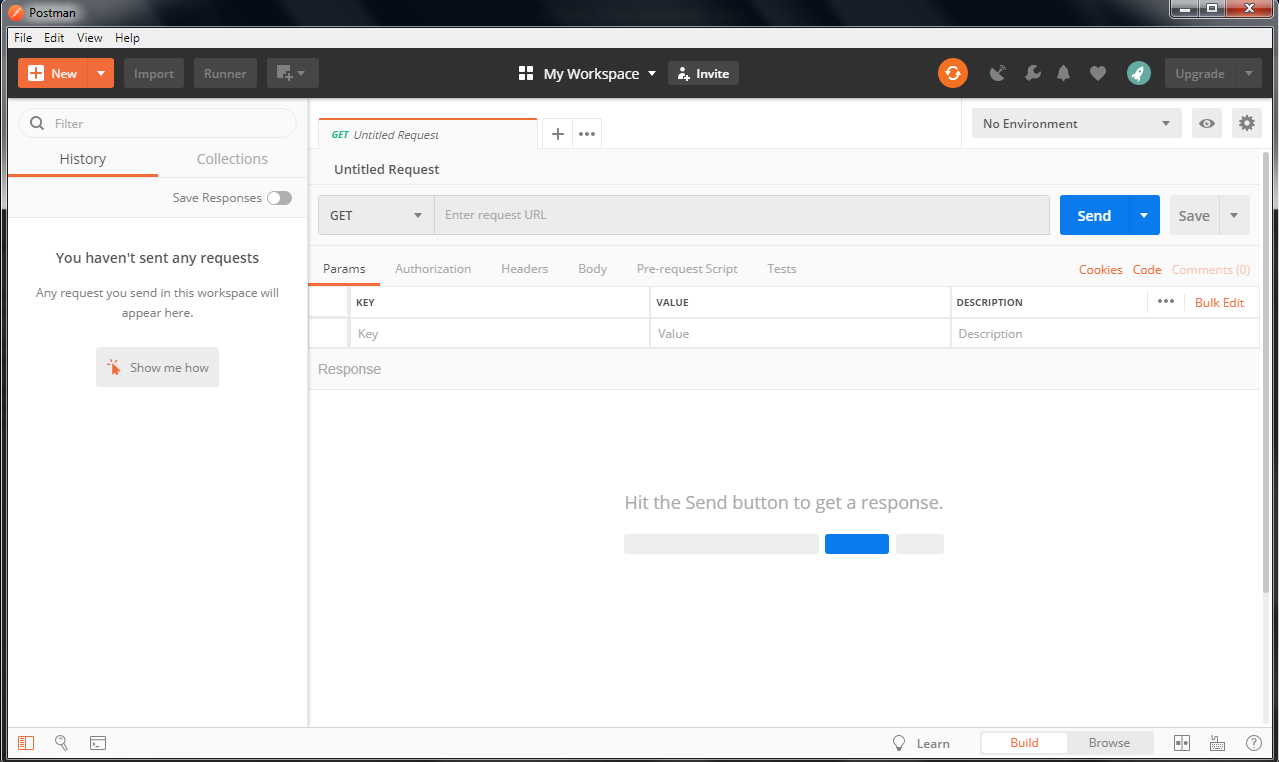
\includegraphics[width=0.85\textwidth]{figures/11/tp.PNG}}
	\caption{Tampilan Postman}
	\label{fig:tp}
\end{figure}
\end{enumerate}

\subsection{Instalasi Ekstensi Postman Pada Web Browser Chrome}
\begin{enumerate}
\item Buka Web store di Chrome dan ketikan Postman. Atau anda dapat melakukan cara lain yaitu dengan melakukan pencarian dengan kata kunci “Postman extension chrome” seperti pada gambar \ref{fig:pepc}.
\begin{figure}[!htbp]
	\centerline{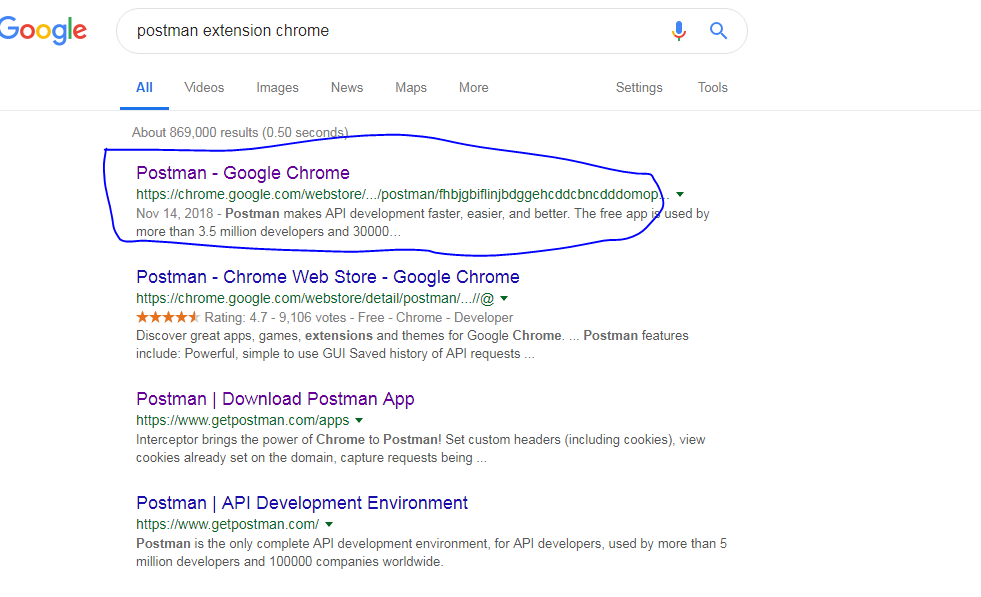
\includegraphics[width=0.85\textwidth]{figures/11/pepc.PNG}}
	\caption{Pencarian Ekstensi Postman Untuk Chrome}
	\label{fig:pepc}
\end{figure}

\item Klik tautan yang dilingkari biru dan akan muncul halaman berikut untuk mengunduh file ekstensinya. Dan klik Add To Chrome untuk memulai pengunduhan seperti pada gambar \ref{fig:pec}.
\begin{figure}[!htbp]
	\centerline{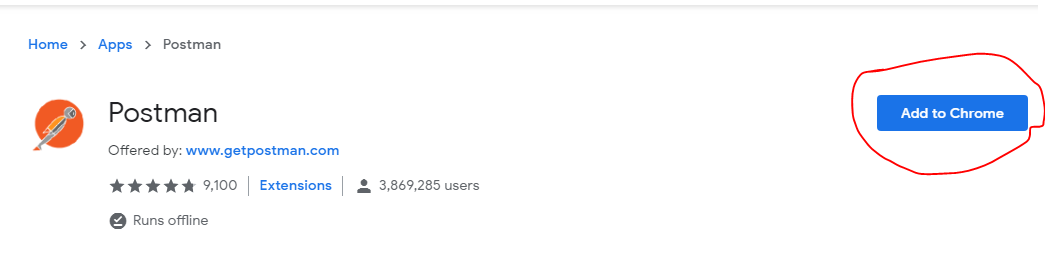
\includegraphics[width=0.85\textwidth]{figures/11/pec.PNG}}
	\caption{Menambahkan Postman ke Ekstensi Chrome}
	\label{fig:pec}
\end{figure}

\item Setelah proses instalasi berhasil, anda akan diarahkan ke laman Apps pada Chrome dan terdapat Ikon Postman yang menandakan bahwa Postman telah terinstal seperti pada gambar \ref{fig:ipc}.
\begin{figure}[!htbp]
	\centerline{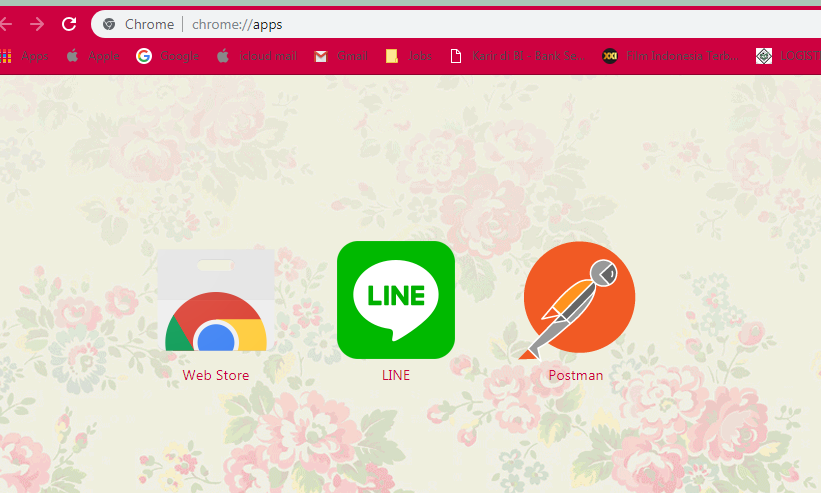
\includegraphics[width=0.85\textwidth]{figures/11/ipc.PNG}}
	\caption{Ikon Postman Pada Laman App Chrome}
	\label{fig:ipc}
\end{figure}
\end{enumerate}

\subsection{Cara Penggunaan Postman Untuk Pengujian HTTP POST,PUT, Dan DELETE}
\begin{enumerate}
\item Pada cmd, jalankan file dari aplikasi yang berisi metode POST,PUT, dan DELETE seperti pada gambar \ref{fig:jac}.
\begin{figure}[!htbp]
	\centerline{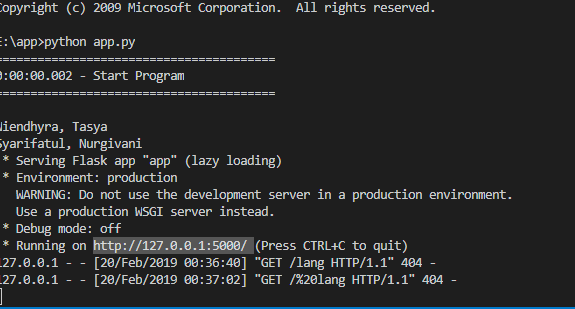
\includegraphics[width=0.85\textwidth]{figures/11/jac.PNG}}
	\caption{Menjalankan Aplikasi Pada CMD}
	\label{fig:jac}
\end{figure}

\item Didapatkan Link yang akan berfungsi untuk menjalankan/ pengujian HTTP Methods yang telah didefinisikan tadi.
\item Buka Postman lalu masukan URL request yang didapatkan tadi dengan menambahkan URL yang telah ditautkan pad fungsi yang telah didefinisikan seperti pada gambar \ref{fig:upm}.
\begin{figure}[!htbp]
	\centerline{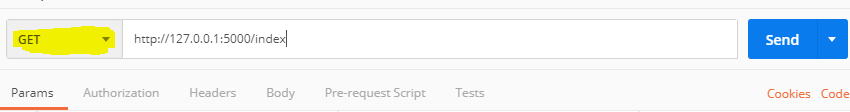
\includegraphics[width=0.85\textwidth]{figures/11/upm.PNG}}
	\caption{Menambahkan URL Untuk POST Method}
	\label{fig:upm}
\end{figure}

\item Pada gambar yang diberi tanda highlight diubah sesuai dengan metode HTTP yang digunakan. Kemudia diubah menjadi POST untuk melakukan pengujian terhadap metode HTTP POST seperti pada gambar \ref{fig:urp}.
\begin{figure}[!htbp]
	\centerline{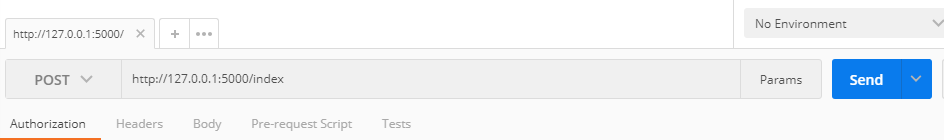
\includegraphics[width=0.85\textwidth]{figures/11/urp.PNG}}
	\caption{Mengubah Request Menjadi POST}
	\label{fig:urp}
\end{figure}

\item Kemudian klik send dan akan muncul seperti ini yang menandakan bahwa metodenya berjalan seperti pada gambar \ref{fig:hppm}.
\begin{figure}[!htbp]
	\centerline{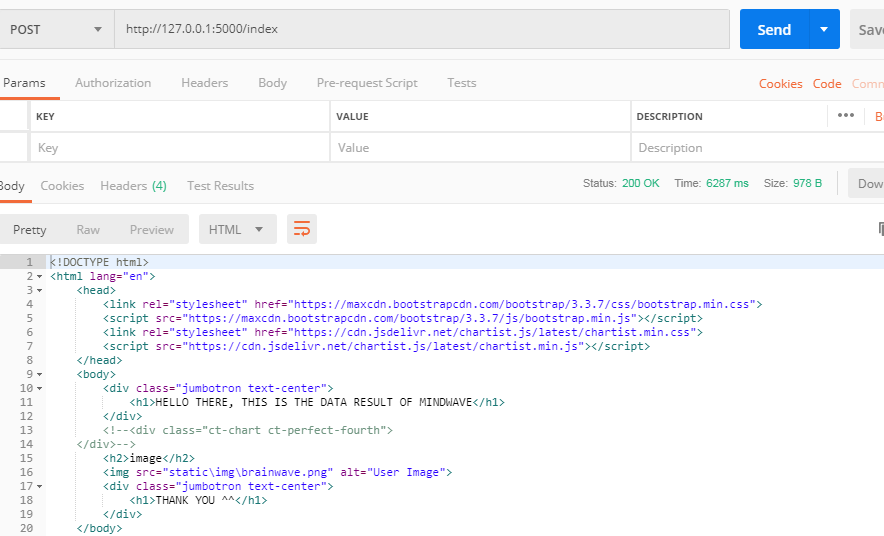
\includegraphics[width=0.85\textwidth]{figures/11/hppm.PNG}}
	\caption{Hasil Pengujian Post Method}
	\label{fig:hppm}
\end{figure}

\item Klik Preview, maka akan tampil laman sesuai dengan yang ada pada web broser, namun gambarnya tidak akan tampil seperti pada gambar \ref{fig:pppm}.
\begin{figure}[!htbp]
	\centerline{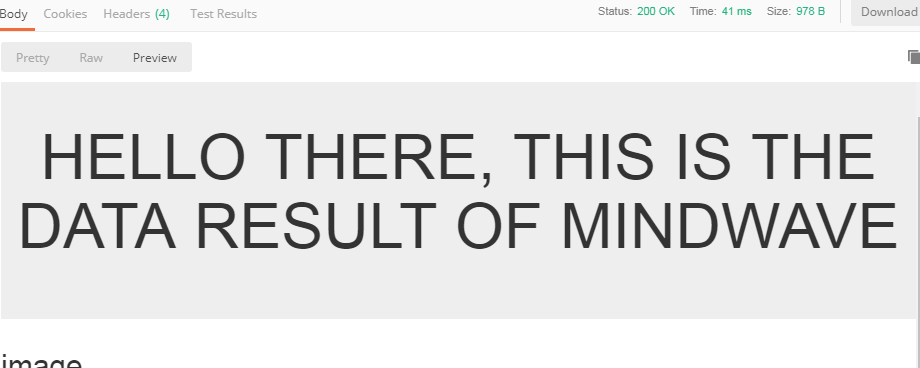
\includegraphics[width=0.85\textwidth]{figures/11/pppm.PNG}}
	\caption{Preview Pengujian Post Method}
	\label{fig:pppm}
\end{figure}

\item Sekarang akan dilakukan pengujian pada metode PUT. Yang dimana akan meng Update data.
\item Pertama – tama jalankan GET Request untuk mendapatkan data yang ingin di update seperti pada gambar \ref{fig:gr}.
\begin{figure}[!htbp]
	\centerline{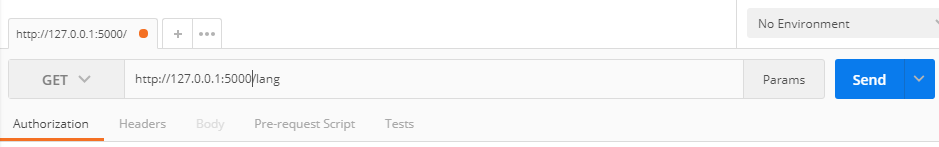
\includegraphics[width=0.85\textwidth]{figures/11/gr.PNG}}
	\caption{Get Request}
	\label{fig:gr}
\end{figure}

Hasilnya seperti pada gambar \ref{fig:hpgr}.
\begin{figure}[!htbp]
	\centerline{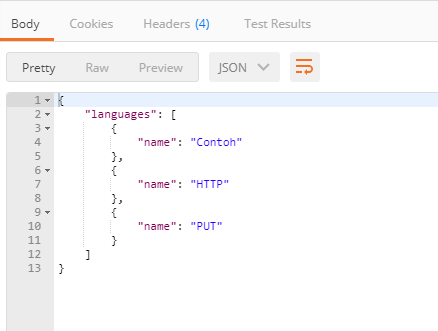
\includegraphics[width=0.85\textwidth]{figures/11/hpgr.PNG}}
	\caption{Hasil Pengujian Get Request}
	\label{fig:hpgr}
\end{figure}

\item Pada Step ini akan mengupdate data “Contoh” mejadi kata lain. Pada bagian URL tambahkan /Contoh yang artinya akan mengedit data tersebut, dan ubah Method Requestnya menjadi PUT. Namun jangan di klik Send seperti pada gambar \ref{fig:cpm}.
\begin{figure}[!htbp]
	\centerline{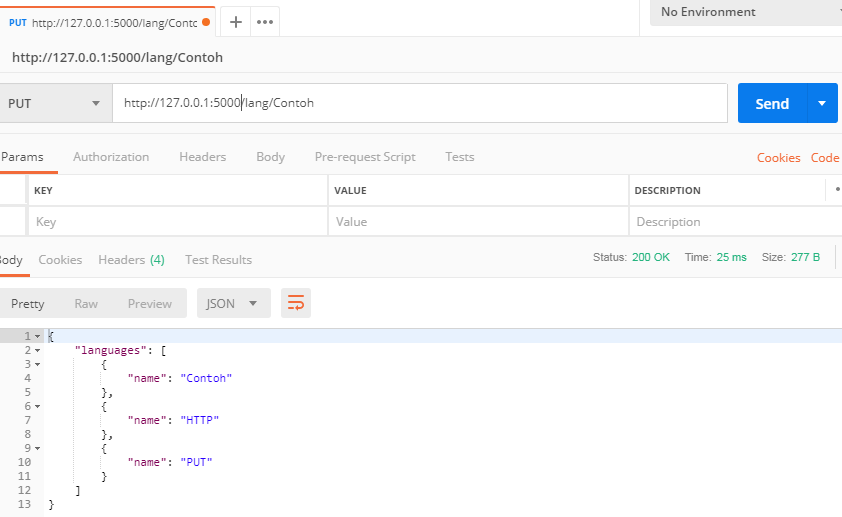
\includegraphics[width=0.85\textwidth]{figures/11/cpm.PNG}}
	\caption{Contoh Put Method}
	\label{fig:cpm}
\end{figure}

\item Pilih Body kemudian pilih Raw dan ketikan seperti dibawah ini. Dan setelah itu klik send. Pastikan Requestnya sudah diganti dengan JSON(applications/json) seperti pada gambar \ref{fig:edc}.
\begin{figure}[!htbp]
	\centerline{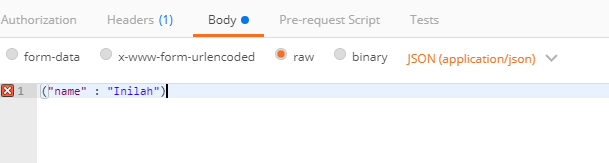
\includegraphics[width=0.85\textwidth]{figures/11/edc.PNG}}
	\caption{Edit Data Contoh}
	\label{fig:edc}
\end{figure}

\item Apabila berhasil maka akan muncul seperti ini yang menandakan bahwa data berhasil di update seperti pada gambar \ref{fig:dct}.
\begin{figure}[!htbp]
	\centerline{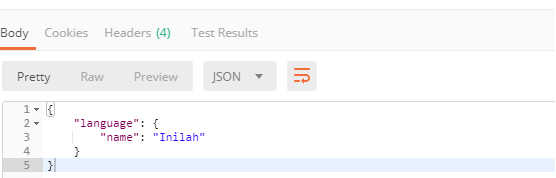
\includegraphics[width=0.85\textwidth]{figures/11/dct.PNG}}
	\caption{Data Contoh Terupdate}
	\label{fig:dct}
\end{figure}

\item Untuk memastikan apakah data benar benar ter update maka jalankan kembali URL http://127.0.0.1:5000/lang pada Postman dengan metode GET. Maka akan terlihat Data yang sebelumnya “Contoh” berubah menjadi “Inilah” seperti pada gambar \ref{fig:dcu}.
\begin{figure}[!htbp]
	\centerline{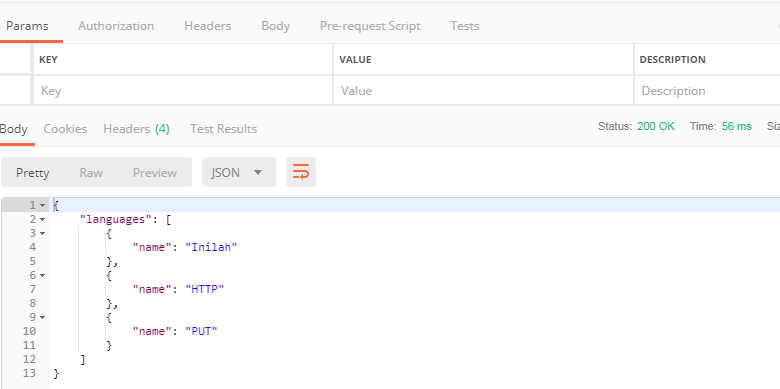
\includegraphics[width=0.85\textwidth]{figures/11/dcu.PNG}}
	\caption{Data Contoh Yang Terupdate}
	\label{fig:dcu}
\end{figure}
 
\item Selanjutnya akan mencoba mengupdate data “HTTP” mejadi kata lain. Untuk itu Pilih Body kemudian pilih Raw dan ketikan seperti dibawah ini. Dan setelah itu klik send seperti pada gambar \ref{fig:edh}.
\begin{figure}[!htbp]
	\centerline{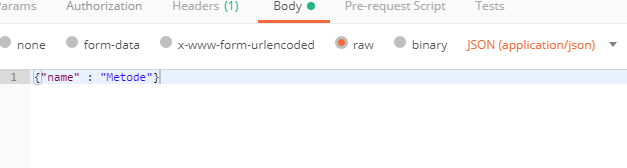
\includegraphics[width=0.85\textwidth]{figures/11/edh.PNG}}
	\caption{Edit Data HTTP}
	\label{fig:edh}
\end{figure}

\item Apabila berhasil maka akan muncul seperti ini yang menandakan bahwa data berhasil di update seperti pada gambar \ref{fig:dht}.
\begin{figure}[!htbp]
	\centerline{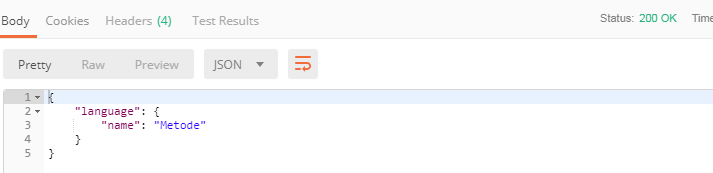
\includegraphics[width=0.85\textwidth]{figures/11/dht.PNG}}
	\caption{Data HTTP Terupdate}
	\label{fig:dht}
\end{figure}
 
\item Untuk memastikan apakah data benar benar ter update maka jalankan kembali URL http://127.0.0.1:5000/lang pada Postman dengan metode GET. Maka akan terlihat Data yang sebelumnya “HTTP” berubah menjadi “Metode” seperti pada gambar \ref{fig:dhu}.
\begin{figure}[!htbp]
	\centerline{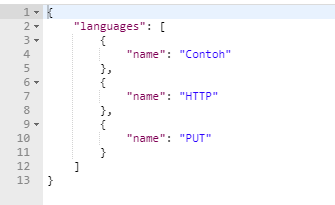
\includegraphics[width=0.85\textwidth]{figures/11/dhu.PNG}}
	\caption{Data HTTP Yang Terupdate}
	\label{fig:dhu}
\end{figure}
 
\item Berikutnya pengujian terhadap HTTP DELETE.
\item Pada Postman ketikan URL http://127.0.0.1:5000/lang/Inilah . Artinya data Inilah dipilih untuk dihapus dari resource seperti pada gambar \ref{fig:uhd}.
\begin{figure}[!htbp]
	\centerline{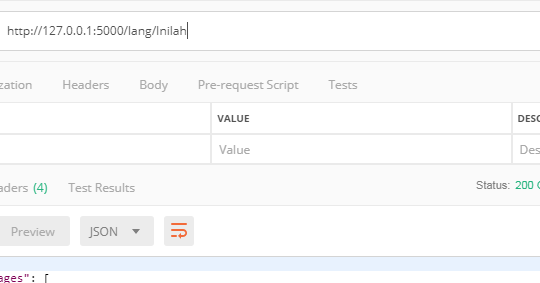
\includegraphics[width=0.85\textwidth]{figures/11/uhd.PNG}}
	\caption{Mengubah URL Untuk HTTP Delete}
	\label{fig:uhd}
\end{figure}

\item Ubah metodenya menjadi DELETE seperti pada gambar \ref{fig:umd}.
\begin{figure}[!htbp]
	\centerline{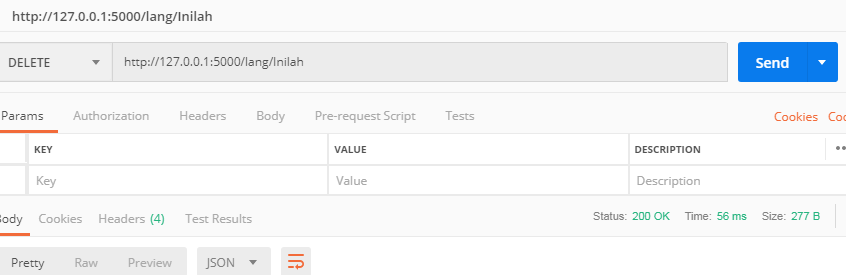
\includegraphics[width=0.85\textwidth]{figures/11/umd.PNG}}
	\caption{Mengubah Metode Menjadi Delete}
	\label{fig:umd}
\end{figure}
 
\item Klik send, dan jika berhasil maka akan seperti ini seperti pada gambar \ref{fig:dt}.
\begin{figure}[!htbp]
	\centerline{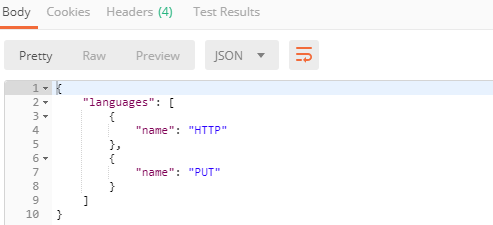
\includegraphics[width=0.85\textwidth]{figures/11/dt.PNG}}
	\caption{Data Inilah Terhapus}
	\label{fig:dt}
\end{figure}
 
\item Untuk memastikan data telah terhapus atau tidak. Lakukan Penghapusan data lagi. Dan akan mencoba menghapus data “HTTP”.
\item Pada Postman ketikan URL http://127.0.0.1:5000/lang/HTTP seperti pada gambar \ref{fig:udh}.
\begin{figure}[!htbp]
	\centerline{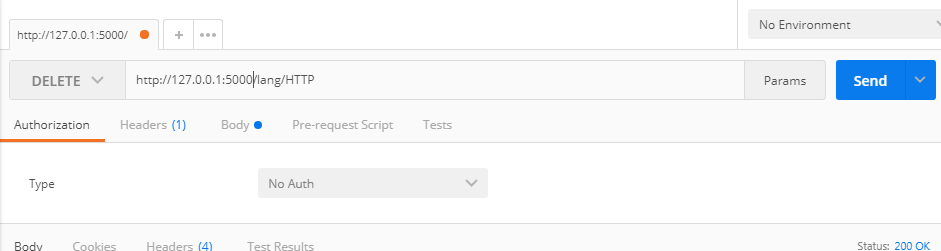
\includegraphics[width=0.85\textwidth]{figures/11/udh.PNG}}
	\caption{Mengubah URL Untuk Delete Data HTTP}
	\label{fig:udh}
\end{figure}

\item Klik send, dan jika berhasil maka akan seperti ini seperti pada gambar \ref{fig:dhh}.
\begin{figure}[!htbp]
	\centerline{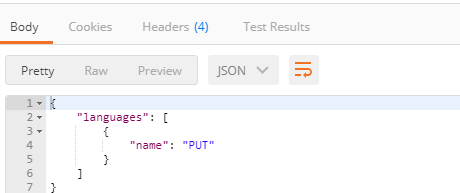
\includegraphics[width=0.85\textwidth]{figures/11/dhh.PNG}}
	\caption{Data HTTP Terhapus}
	\label{fig:dhh}
\end{figure}
\end{enumerate}

\section{Penanganan Error}
\subsection{TypeError: 'NoneType' Object Has No Attribute}
Errornya seperti pada gambar \ref{fig:nte}.
\begin{figure}[!htbp]
	\centerline{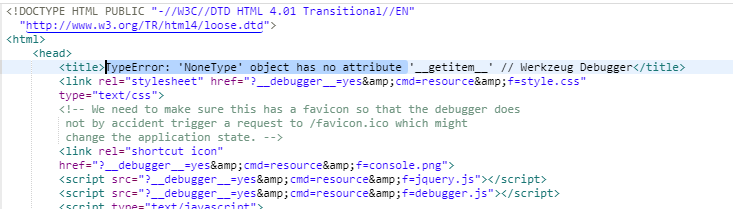
\includegraphics[width=0.85\textwidth]{figures/11/nte.PNG}}
	\caption{TypeError: 'NoneType' Object Has No Attribute}
	\label{fig:nte}
\end{figure}

Error ini biasanya terjadi pada saat mengedit  Body untuk menambahkan atau memperbarui data. Eror ini menandakan bahwa NoneType berarti bahwa alih-alih sebuah instance dari Kelas atau Obyek apa pun yang Anda pikir sedang dikerjakan, sebenarnya tidak anda miliki satupun. Itu biasanya berarti bahwa tugas atau fungsi panggilan di atas gagal atau mengembalikan hasil yang tidak terduga.

Cara Mengatasi Error:
\begin{enumerate}
\item Buka Postman seperti pada gambar \ref{fig:jp}.
\begin{figure}[!htbp]
	\centerline{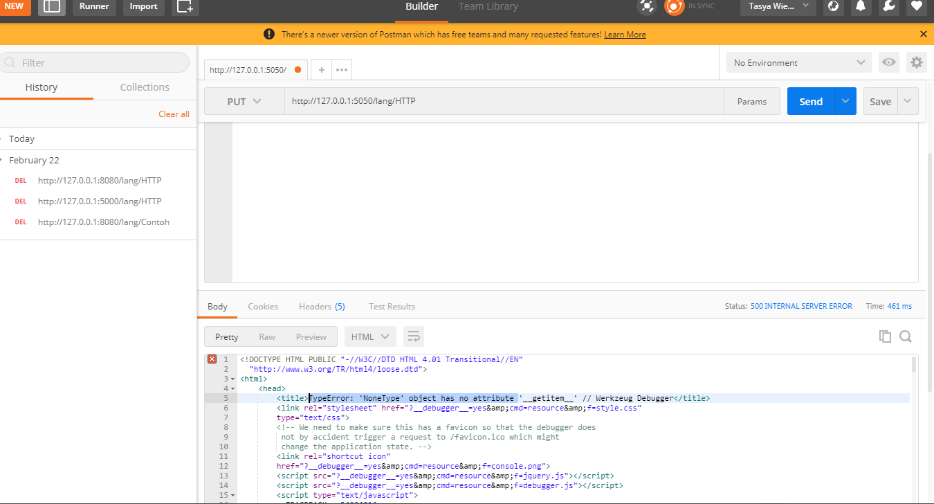
\includegraphics[width=0.85\textwidth]{figures/11/jp.PNG}}
	\caption{Menjalankan Postman}
	\label{fig:jp}
\end{figure}

\item Ubah Objek metode menjadi ‘PUT’ dan pilih Data yang akan diupdate atau menambahkan data baru seperti pada gambar \ref{fig:um}.
\begin{figure}[!htbp]
	\centerline{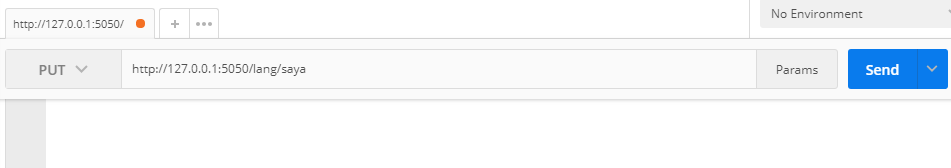
\includegraphics[width=0.85\textwidth]{figures/11/um.PNG}}
	\caption{Mengubah Metode}
	\label{fig:um}
\end{figure}

\item Setelah itu, pilih Body seperti pada gambar \ref{fig:mbp}.
\begin{figure}[!htbp]
	\centerline{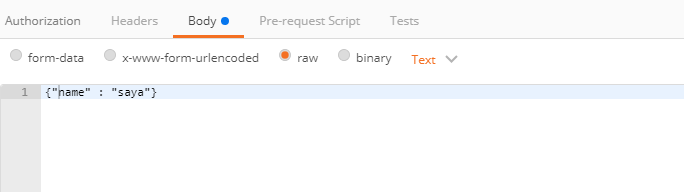
\includegraphics[width=0.85\textwidth]{figures/11/mbp.PNG}}
	\caption{Memilih Body Pada Postman}
	\label{fig:mbp}
\end{figure}

\item Dari gambar diatas, diketahui bahwa objek type nya masih ‘TEXT. Maka dari itu klik pada bagian tersebut, dan ubah menjadi json, seperti pada gambar \ref{fig:mot}.
\begin{figure}[!htbp]
	\centerline{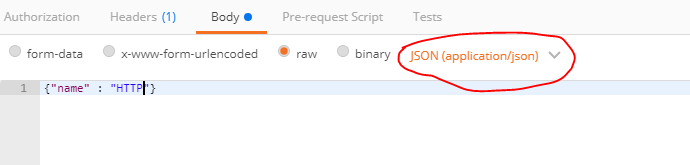
\includegraphics[width=0.85\textwidth]{figures/11/mot.PNG}}
	\caption{Mengubah Object Type}
	\label{fig:mot}
\end{figure}

\item Ubah juga isi dari body seperti gambar diatas. Maka ketika dijalankan, data Saya akan berubah menjadi ‘HTTP’ seperti pada gambar \ref{fig:pu}.
\begin{figure}[!htbp]
	\centerline{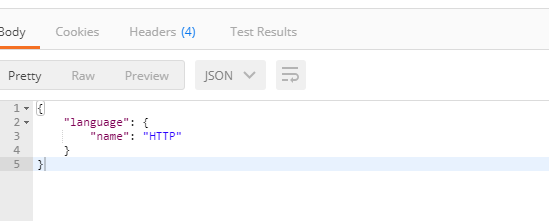
\includegraphics[width=0.85\textwidth]{figures/11/pu.PNG}}
	\caption{Pengujian}
	\label{fig:pu}
\end{figure}
\end{enumerate}

\subsection{DELETE Error Code 404} 
Delete Error Code 404 seperti pada gambar \ref{fig:dec}.
\begin{figure}[!htbp]
	\centerline{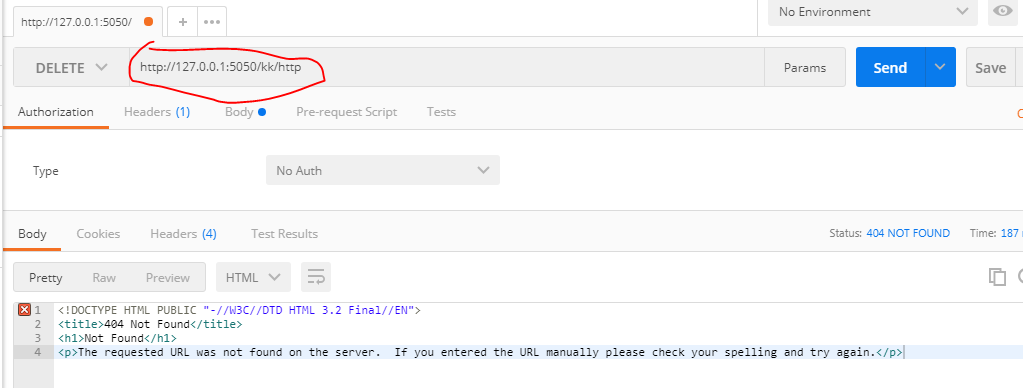
\includegraphics[width=0.85\textwidth]{figures/11/dec.PNG}}
	\caption{DELETE Error Code 404}
	\label{fig:dec}
\end{figure}

Pada tutorial ini menerima 404 karena / kk/ HTTP bukan URI yang menunjuk ke sumber daya di sistem. Idempotensi juga dipertahankan karena berapa kali Anda mengirim permintaan HTTP DELETE ini, perubahan tambahan ke kondisi server tidak akan terjadi karena sumber daya sudah dihapus. Jadi, permintaan HTTP DELETE tambahan tidak akan melakukan apa-apa.

Cara Mengatasi Error:
\begin{enumerate} 
\item Untuk eror ini sangat mudah dalam penyelesaiannya. Cukup dengan mengubah URI ke sumber daya di sistem.
\item URI pada sistem tutorial ini seperti pada gambar \ref{fig:uus}.
\begin{figure}[!htbp]
	\centerline{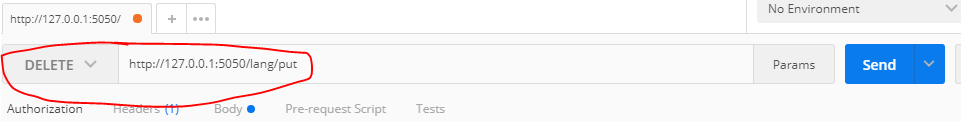
\includegraphics[width=0.85\textwidth]{figures/11/uus.PNG}}
	\caption{Mengubah URI Sesuai Dengan Sistem}
	\label{fig:uus}
\end{figure}

\item Setelah diubah, klik Send. Maka data ‘PUT’ akan terhapus seperti pada gambar \ref{fig:dsd}.
\begin{figure}[!htbp]
	\centerline{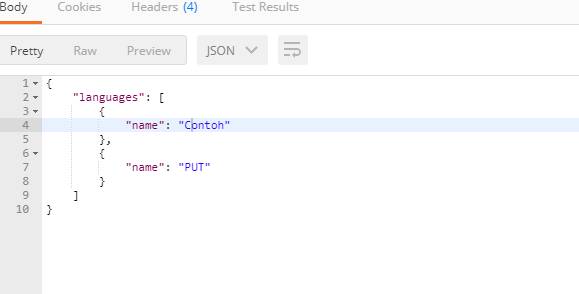
\includegraphics[width=0.85\textwidth]{figures/11/dsd.PNG}}
	\caption{Data Sebelum Dihapus}
	\label{fig:dsd}
\end{figure}

Data setelah dihapus seperti pada gambar \ref{fig:dsh}.
\begin{figure}[!htbp]
	\centerline{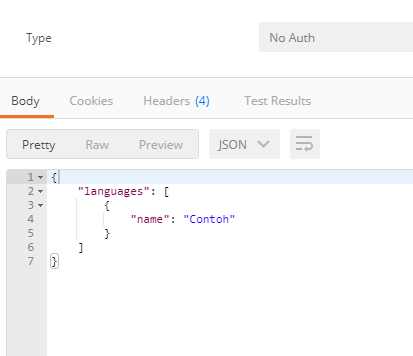
\includegraphics[width=0.85\textwidth]{figures/11/dsh.PNG}}
	\caption{Data Setelah Dihapus}
	\label{fig:dsh}
\end{figure}
\end{enumerate}